\documentclass{beamer}
\mode<presentation>
\usepackage{amsmath}
\usepackage{amssymb}
%\usepackage{advdate}
\usepackage{adjustbox}
\usepackage{subcaption}
\usepackage{enumitem}
\usepackage{multicol}
\usepackage{mathtools}
\usepackage{listings}
\usepackage{float}
\newcommand{\rank}{\operatorname{rank}}
\usepackage{graphicx}
\usepackage{url}
\def\UrlBreaks{\do\/\do-}
\usetheme{Boadilla}
\usecolortheme{lily}
\setbeamertemplate{footline}
{
  \leavevmode%
  \hbox{%
  \begin{beamercolorbox}[wd=\paperwidth,ht=2.25ex,dp=1ex,right]{author in head/foot}%
    \insertframenumber{} / \inserttotalframenumber\hspace*{2ex} 
  \end{beamercolorbox}}%
  \vskip0pt%
}
\setbeamertemplate{navigation symbols}{}

\providecommand{\nCr}[2]{\,^{#1}C_{#2}} % nCr
\providecommand{\nPr}[2]{\,^{#1}P_{#2}} % nPr
\providecommand{\mbf}{\mathbf}
\providecommand{\pr}[1]{\ensuremath{\Pr\left(#1\right)}}
\providecommand{\qfunc}[1]{\ensuremath{Q\left(#1\right)}}
\providecommand{\sbrak}[1]{\ensuremath{{}\left[#1\right]}}
\providecommand{\lsbrak}[1]{\ensuremath{{}\left[#1\right.}}
\providecommand{\rsbrak}[1]{\ensuremath{{}\left.#1\right]}}
\providecommand{\brak}[1]{\ensuremath{\left(#1\right)}}
\providecommand{\lbrak}[1]{\ensuremath{\left(#1\right.}}
\providecommand{\rbrak}[1]{\ensuremath{\left.#1\right)}}
\providecommand{\cbrak}[1]{\ensuremath{\left\{#1\right\}}}
\providecommand{\lcbrak}[1]{\ensuremath{\left\{#1\right.}}
\providecommand{\rcbrak}[1]{\ensuremath{\left.#1\right\}}}
\theoremstyle{remark}
\newtheorem{rem}{Remark}
\newcommand{\sgn}{\mathop{\mathrm{sgn}}}
\providecommand{\abs}[1]{\left\vert#1\right\vert}
\providecommand{\res}[1]{\Res\displaylimits_{#1}} 
\providecommand{\norm}[1]{\lVert#1\rVert}
\providecommand{\mtx}[1]{\mathbf{#1}}
\providecommand{\mean}[1]{E\left[ #1 \right]}
\providecommand{\fourier}{\overset{\mathcal{F}}{ \rightleftharpoons}}
%\providecommand{\hilbert}{\overset{\mathcal{H}}{ \rightleftharpoons}}
\providecommand{\system}{\overset{\mathcal{H}}{ \longleftrightarrow}}
	%\newcommand{\solution}[2]{\textbf{Solution:}{#1}}
%\newcommand{\solution}{\noindent \textbf{Solution: }}
\providecommand{\dec}[2]{\ensuremath{\overset{#1}{\underset{#2}{\gtrless}}}}
\newcommand{\myvec}[1]{\ensuremath{\begin{pmatrix}#1\end{pmatrix}}}
\let\vec\mathbf

\lstset{
language=C,
frame=single, 
breaklines=true,
columns=fullflexible
}

\numberwithin{equation}{section}

\title{Presentation - Matgeo}
\author{Aryansingh Sonaye \\
AI25BTECH11032 \\
EE1030 - Matrix Theory}

\date{\today} 
\begin{document}

\begin{frame}
\titlepage
\end{frame}

\section{Problem}
\begin{frame}
\frametitle{Problem Statement}
\textbf{Problem (4.4.28) :} The $x$-coordinate of a point on the line joining the points 
$\vec{P}(2,2,1)$ and $\vec{Q}(5,1,-2)$ is $4$. Find its $z$-coordinate.
\end{frame}

\section{Solution}
\subsection{Description of Variables used}
\begin{frame}
\frametitle{Description of Variables used}
\begin{table}[H]
\centering
\begin{tabular}[12pt]{ |c| c|}
    \hline
    \textbf{Input variable} & \textbf{Value}\\ 
    \hline
    $\vec{P}$ & \myvec{2 \\2 \\1} \\
    \hline 
    $\vec{Q}$ & \myvec{5 \\1 \\-2}\\
    \hline
    $\vec{R}$ & \myvec{4 \\y \\z}\\
    \hline
    \end{tabular}
    \caption{}
    \label{}
 \end{table}


\end{frame}

\subsection{Theoretical Solution }

\begin{frame}
\frametitle{Theoretical Solution}
Form the column vectors $\vec{Q-P}$ and $\vec{R-P}$ and the matrix $\vec{M}$ whose columns are these vectors:
\begin{align}
\vec{Q-P} &= \myvec{3\\-1\\-3}, & \vec{R-P} &= \myvec{2\\y-2\\z-1},\\[6pt]
\vec{M} &= \myvec{3 & 2 \\ -1 & y-2 \\ -3 & z-1}.
\end{align}

Take the transpose $\vec{M^{\!T}}$ :
\begin{align}
\vec{M^{\!T}} &= \myvec{3 & -1 & -3 \\[4pt] 2 & y-2 & z-1 }.
\end{align}
\end{frame}

\begin{frame}
\frametitle{Theoretical Solution}
Perform the row operation \(R_2 \leftarrow R_2 - \tfrac{2}{3}R_1\).  Writing the entries explicitly gives
\begin{align}
R_1 &\;=\; \myvec{3 & -1 & -3}, \\[4pt]
R_2 &\;=\; \myvec{2 & y-2 & z-1} - \tfrac{2}{3}\myvec{3 & -1 & -3} \\[4pt]
 R_2 &    \;=\; \myvec{2 - \tfrac{2}{3}\cdot 3 \; &\; (y-2) - \tfrac{2}{3}\cdot(-1) \; &\; (z-1) - \tfrac{2}{3}\cdot(-3)}.
\end{align}

Thus after the row operation we have
\begin{align}
\vec{M^{\!T}}_{\text{after}} \;=\;
\myvec{
3 & -1 & -3 \\[4pt]
2 - \tfrac{2}{3}\cdot 3 & (y-2) - \tfrac{2}{3}\cdot(-1) & (z-1) - \tfrac{2}{3}\cdot(-3)
}
\end{align}

\end{frame}

\begin{frame}
\frametitle{Theoretical Solution}
Carry out the indicated multiplications to simplify the entries of the second row:
\begin{align}
2 - \tfrac{2}{3}\cdot 3 &= 2 - 2 = 0,\\[4pt]
(y-2) - \tfrac{2}{3}\cdot(-1) &= y - 2 + \tfrac{2}{3} = y - \tfrac{4}{3},\\[4pt]
(z-1) - \tfrac{2}{3}\cdot(-3) &= z - 1 + 2 = z + 1.
\end{align}

So the fully simplified matrix after the row operation is
\begin{align}
\vec{M^{\!T}}_{\text{after}} \;=\;
\myvec{
3 & -1 & -3 \\[4pt]
0 & y - \tfrac{4}{3} & z + 1
}
\end{align}


\end{frame}

\begin{frame}
\frametitle{Theoretical Solution}
For the columns of $M$ to be linearly dependent (equivalently for $P,Q,R$ to be collinear) we require $\rank(M)=1$.  Since $\rank(\vec{M})=\rank(\vec{M^{\!T}})$, and $\vec{M^{\!T}}_{\text{after}}$ has two rows, rank $=1$ means the second row must be the zero row. Hence
\begin{align}
y - \tfrac{4}{3} &= 0,\\
z + 1 &= 0.
\end{align}

Therefore
\begin{align}
y &= \tfrac{4}{3}, & z &= -1.
\end{align}

\begin{align}
\boxed{z = -1}
\end{align}
\end{frame}

\subsection{Plot}
\begin{frame}
    \frametitle{Plot}
\begin{figure}[H]
   \centering
   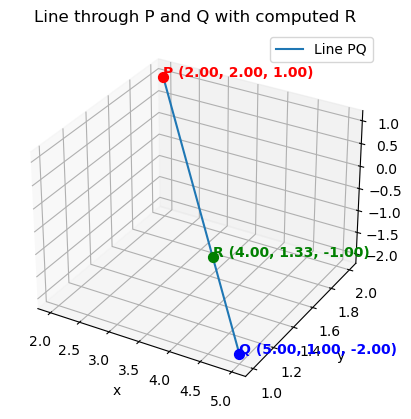
\includegraphics[width=0.6\columnwidth]{figs/line_3d.png}
   \end{figure}
\end{frame}

\begin{frame}[fragile]
    \frametitle{Code - C}
    \begin{lstlisting}
#include <stdio.h>

/* Compute multiplier = a21 / a11.
   If a11 == 0, print "Error" and return 0.0 .
*/
double compute_multiplier(double a11, double a21) {
    if (a11 == 0.0) {
        printf("Error\n");
        return 0.0;
    }
    return a21 / a11;
}


\end{lstlisting}
\end{frame}

\begin{frame}[fragile]
\frametitle{Code - C}
\begin{lstlisting}
/* Perform row op: out2[j] = r2[j] - (r2[0]/r1[0]) * r1[j] for j=0..2
   If r1[0] == 0, print "Error" and set out2 to zeros.
*/
void apply_row_op(const double r1[3], const double r2[3], double out2[3]) {
    if (r1[0] == 0.0) {
        printf("Error\n");
        out2[0] = out2[1] = out2[2] = 0.0;
        return;
    }
    double mult = r2[0] / r1[0];
    for (int j = 0; j < 3; ++j) {
        out2[j] = r2[j] - mult * r1[j];
    }
}


\end{lstlisting}
\end{frame}

\begin{frame}[fragile]
    \frametitle{Code - Python(with shared C code)}
    \begin{lstlisting}
import ctypes
from ctypes import c_double
import numpy as np
import matplotlib.pyplot as plt
from mpl_toolkits.mplot3d import Axes3D  # registers 3D projection

# ---------- User inputs ----------
P = (2.0, 2.0, 1.0)   # Px,Py,Pz
Q = (5.0, 1.0, -2.0)  # Qx,Qy,Qz
Rx_given = 4.0        # given x-coordinate of R

# ---------- compute direction D = Q - P ----------
Px, Py, Pz = P
Qx, Qy, Qz = Q
Dx = Qx - Px
Dy = Qy - Py
Dz = Qz - Pz


\end{lstlisting}
\end{frame}
\begin{frame}[fragile]
\frametitle{Code - Python(with shared C code)}
\begin{lstlisting}
if abs(Dx) < 1e-12:
    raise SystemExit("Error: Dx = 0. This script pivots on x; please pick a case with Dx != 0.")
# ---------- load C shared lib ----------
lib = ctypes.CDLL('./librow.so')
lib.compute_multiplier.argtypes = (c_double, c_double)
lib.compute_multiplier.restype = c_double
lib.apply_row_op.argtypes = (ctypes.POINTER(c_double),
                             ctypes.POINTER(c_double),
                             ctypes.POINTER(c_double))
lib.apply_row_op.restype = None
# ---------- call compute_multiplier in C ----------
a11 = float(Dx)              # r1[0]
a21 = float(Rx_given - Px)   # r2[0]
mult = lib.compute_multiplier(c_double(a11), c_double(a21))
print("Multiplier (from C) =", mult)

\end{lstlisting}
\end{frame}

\begin{frame}[fragile]
\frametitle{Code - Python(with shared C code)}
\begin{lstlisting}
# ---------- compute y and z ----------
t = mult
y = Py + t * Dy
z = Pz + t * Dz
R = (Rx_given, y, z)
print("Computed R =", R)

# ---------- verify using apply_row_op ----------
r1 = (c_double * 3)(Dx, Dy, Dz)
r2 = (c_double * 3)(Rx_given - Px, y - Py, z - Pz)
out2 = (c_double * 3)()
lib.apply_row_op(r1, r2, out2)
out_list = [float(out2[i]) for i in range(3)]
print("Second row after elimination (from C apply_row_op):", out_list)


\end{lstlisting}
\end{frame}

\begin{frame}[fragile]
\frametitle{Code - Python(with shared C code)}
\begin{lstlisting}
# ---------- plot P, Q, R with labels ----------
N = 101
ts = np.linspace(0.0, 1.0, N)
points = np.array([[Px + t*Dx, Py + t*Dy, Pz + t*Dz] for t in ts])

img3d = "line_3d.png"
fig = plt.figure()
ax = fig.add_subplot(111, projection='3d')

# line PQ
ax.plot(points[:,0], points[:,1], points[:,2], label='Line PQ')

# helper to format coordinates
def fmt_coords(pt):
    return f"({pt[0]:.2f}, {pt[1]:.2f}, {pt[2]:.2f})"

\end{lstlisting}
\end{frame}

\begin{frame}[fragile]
\frametitle{Code - Python(with shared C code)}
\begin{lstlisting}
# points + labels
ax.scatter(*P, color='red', s=50)
ax.text(*P, f"P {fmt_coords(P)}", color='red', fontsize=10, weight='bold')

ax.scatter(*Q, color='blue', s=50)
ax.text(*Q, f"Q {fmt_coords(Q)}", color='blue', fontsize=10, weight='bold')

ax.scatter(*R, color='green', s=50)
ax.text(*R, f"R {fmt_coords(R)}", color='green', fontsize=10, weight='bold')

\end{lstlisting}
\end{frame}

\begin{frame}[fragile]
\frametitle{Code - Python(with shared C code)}
\begin{lstlisting}
ax.set_xlabel('x')
ax.set_ylabel('y')
ax.set_zlabel('z')
ax.set_title('Line through P and Q with computed R')
plt.legend()

# save and show
plt.savefig(img3d, bbox_inches='tight')
print("Saved 3D image with P, Q, R labels ->", img3d)
plt.show()

\end{lstlisting}
\end{frame}

\begin{frame}[fragile]
\frametitle{Code - Python only}
\begin{lstlisting}
import numpy as np
import matplotlib.pyplot as plt
from mpl_toolkits.mplot3d import Axes3D  # registers 3D projection

# ---------- Problem data (change if you want to test other examples) ----------
P = (2.0, 2.0, 1.0)    # (Px, Py, Pz)
Q = (5.0, 1.0, -2.0)   # (Qx, Qy, Qz)
Rx_given = 4.0         # known x-coordinate of R (we pivot on x here)
# ---------- helper: row operation in Python ----------
def apply_row_op_py(r1, r2):
    """
    Perform R2 <- R2 - mult * R1 where mult = r2[0] / r1[0].
    r1, r2 are length-3 iterables of numbers.
    Returns (mult, new_r2) where new_r2 is a list of 3 floats.
    If r1[0] == 0, raises ValueError.
    """
\end{lstlisting}
\end{frame}
\begin{frame}[fragile]
\frametitle{Code - Python only}
\begin{lstlisting}
    a11 = float(r1[0])
    if abs(a11) < 1e-15:
        raise ValueError("Pivot (r1[0]) is zero; cannot eliminate.")
    mult = float(r2[0]) / a11
    new_r2 = [r2[j] - mult * r1[j] for j in range(3)]
    return mult, new_r2

# ---------- compute direction and check pivot ----------
Px, Py, Pz = P
Qx, Qy, Qz = Q
Dx, Dy, Dz = Qx - Px, Qy - Py, Qz - Pz

if abs(Dx) < 1e-12:
    raise SystemExit("Pivot Dx is zero; this script is pivoting on x. Choose different input or pivot axis.")



\end{lstlisting}
\end{frame}

\begin{frame}[fragile]
\frametitle{Code - Python only}
\begin{lstlisting}
# ---------- build M^T rows (numeric with symbolic part in r2 before solving) ----------
# r1 = [Dx, Dy, Dz]
# r2 (before knowing y,z) = [Rx_given - Px, (y-Py), (z-Pz)]
# we will compute t = (Rx_given - Px)/Dx via multiplier
r1 = [Dx, Dy, Dz]
r2_first = Rx_given - Px  # numeric pivot entry
# ---------- get multiplier t (same as parameter) ----------
t = r2_first / Dx   # Exactly same as compute_multiplier
print("Multiplier t = (Rx - Px)/Dx =", t)
# ---------- compute y and z from parametric form X = P + t*D ----------
y = Py + t * Dy
z = Pz + t * Dz
R = (Rx_given, y, z)
print("Computed R = (x, y, z) =", (R[0], R[1], R[2]))

\end{lstlisting}
\end{frame}

\begin{frame}[fragile]
\frametitle{Code - Python only}
\begin{lstlisting}
# ---------- now form numeric second row and apply row op in Python to verify ----------
r2 = [r2_first, y - Py, z - Pz]   # numeric second row now
mult_used, new_r2 = apply_row_op_py(r1, r2)

print("\nRow operation details:")
print(" r1 =", r1)
print(" r2 (before) =", r2)
print(" multiplier used =", mult_used)
print(" r2 (after)  =", new_r2)

# check near-zero
tol = 1e-9
if all(abs(v) < tol for v in new_r2):
    print("Verification: second row reduced to zero (rank = 1) within tolerance.")



\end{lstlisting}
\end{frame}

\begin{frame}[fragile]
\frametitle{Code - Python only}
\begin{lstlisting}
else:
    print("Warning: second row not exactly zero; values:", new_r2)

# ---------- Plotting (3D) with labels and coordinates ----------
def fmt_coords(pt):
    return f"({pt[0]:.2f}, {pt[1]:.2f}, {pt[2]:.2f})"

N = 101
ts = np.linspace(0.0, 1.0, N)
points = np.array([[Px + t*Dx, Py + t*Dy, Pz + t*Dz] for t in ts])

fig = plt.figure()
ax = fig.add_subplot(111, projection='3d')

\end{lstlisting}
\end{frame}

\begin{frame}[fragile]
\frametitle{Code - Python only}
\begin{lstlisting}
# plot the line
ax.plot(points[:,0], points[:,1], points[:,2], label='Line PQ')

# plot points
ax.scatter(*P, color='red', s=60)
ax.text(P[0], P[1], P[2], f"  P {fmt_coords(P)}", color='red', fontsize=10, weight='bold')

ax.scatter(*Q, color='blue', s=60)
ax.text(Q[0], Q[1], Q[2], f"  Q {fmt_coords(Q)}", color='blue', fontsize=10, weight='bold')

ax.scatter(*R, color='green', s=60)
ax.text(R[0], R[1], R[2], f"  R {fmt_coords(R)}", color='green', fontsize=10, weight='bold')

\end{lstlisting}
\end{frame}

\begin{frame}[fragile]
\frametitle{Code - Python only}
\begin{lstlisting}
# optional: draw dashed line from R down to x-y plane to help read z (uncomment if you like)
# ax.plot([R[0], R[0]], [R[1], R[1]], [0, R[2]], linestyle='--', linewidth=1)

ax.set_xlabel('x')
ax.set_ylabel('y')
ax.set_zlabel('z')
ax.set_title('Line through P and Q with computed R')
ax.legend()

# save and show
imgfile = "line_3d_python_only.png"
plt.savefig(imgfile, bbox_inches='tight')
print(f"Saved 3D image: {imgfile}")

plt.show()
\end{lstlisting}
\end{frame}

\end{document}
